
% This LaTeX was auto-generated from MATLAB code.
% To make changes, update the MATLAB code and republish this document.











    
    \begin{DoxyCode}
function example_dirac_secondorder_vectmult()
\end{DoxyCode}
\begin{par}
COMPILATION
\end{par} \vspace{1em}
\begin{DoxyCode}
    [exdir,~,~]=fileparts(which('example_dirac_secondorder_vectmult.m'));
    % compile the model
    amiwrap('model_dirac_secondorder_vectmult','model_dirac_secondorder_vectmult_syms',exdir,2)
\end{DoxyCode}

         \begin{DoxyCode}Generating model struct ...
x | k | p | deltax | xdot | deltaxdot | ddeltaxdx | ddeltaxdp | ddeltaxdt | root | drootdx | sx | drootdp | drootdt | dtaudp | sroot | stau | deltasx | sigma_y | dsigma_ydp | y | dydp | sigma_z | dsigma_zdp | z | dzdp | Parsing model struct ...
z | 

Generating C code ...
deltasx | deltax | dsigma_ydp | dsigma_zdp | dydp | dzdp | root | sigma_y | sigma_z | stau | xdot | y | z | headers | wrapfunctions | 
headers | wrapfunctions | 
Compiling mex file ...
amici | Building with 'Xcode with Clang'.
MEX completed successfully.
Building with 'Xcode with Clang'.
MEX completed successfully.
amici | Building with 'Xcode with Clang'.
MEX completed successfully.
Building with 'Xcode with Clang'.
MEX completed successfully.
\end{DoxyCode} 
    \begin{par}
SIMULATION
\end{par} \vspace{1em}
\begin{DoxyCode}
    % time vector
    t = linspace(0,3,1001);
    p = [1;0.5;2;3];
    k = [];
    v = [0.7;0.3;1.4;0.1];

    options = amioption('sensi',0,...
        'maxsteps',1e4);

    % load mex into memory
    [msg] = which('model_dirac_secondorder_vectmult'); % fix for inaccessability problems
    options.sensi = 2;
    sol = simulate_model_dirac_secondorder_vectmult(t,log10(p),k,[],options,v);
\end{DoxyCode}
\begin{par}
FORWARD SENSITIVITY ANALYSIS
\end{par} \vspace{1em}
\begin{DoxyCode}
    options.sensi = 2;

    sol = simulate_model_dirac_secondorder_vectmult(t,log10(p),k,[],options,v);
\end{DoxyCode}
\begin{par}
FINITE DIFFERENCES
\end{par} \vspace{1em}
\begin{DoxyCode}
    options.sensi = 1;

    eps = 1e-4;
    xi = log10(p);
    for ip = 1:4;
        xip = xi;
        xip(ip) = xip(ip) + eps;
        solp = simulate_model_dirac_secondorder_vectmult(t,xip,k,[],options);
        s2x_fd(:,:,ip) = sum(bsxfun(@times,(solp.sx - sol.sx)/eps,permute(v,[3,2,1])),3);
        s2y_fd(:,:,ip) = sum(bsxfun(@times,(solp.sy - sol.sy)/eps,permute(v,[3,2,1])),3);
    end
\end{DoxyCode}
\begin{par}
PLOTTING
\end{par} \vspace{1em}
\begin{DoxyCode}
    figure
    c_x = get(gca,'ColorOrder');
    for ip = 1:4
        subplot(4,2,ip*2-1)
        hold on
        for ix = 1:size(sol.x,2)
            plot(t,sol.s2x(:,ix,ip),'.-','Color',c_x(ix,:))
            plot(t,s2x_fd(:,ix,ip),'--','Color',c_x(ix,:))
        end
        ylim([-10,10])
        legend('x1','x1_{fd}','x2','x2_{fd}','Location','NorthEastOutside')
        legend boxoff
        title(['state sensitivity for p' num2str(ip)])
        xlabel('time t')
        ylabel('x')
        box on

        subplot(4,2,ip*2)
        plot(t,abs(sol.s2x(:,:,ip)-s2x_fd(:,:,ip)),'r--')
        legend('error x1','error x2','Location','NorthEastOutside')
        legend boxoff
        title(['state sensitivity for p' num2str(ip)])
        xlabel('time t')
        ylabel('error')
        ylim([1e-12,1e0])
        set(gca,'YScale','log')
        box on
    end
    set(gcf,'Position',[100 300 1200 500])

    figure
    for ip = 1:4
        subplot(4,2,ip*2-1)
        hold on
        for iy = 1:size(sol.y,2)
            plot(t,sol.s2y(:,iy,ip),'.-','Color',c_x(iy,:))
            plot(t,s2y_fd(:,iy,ip),'--','Color',c_x(iy,:))
        end
        ylim([-10,10])
        legend('y1','y1_{fd}','Location','NorthEastOutside')
        legend boxoff
        title(['observable sensitivity for p' num2str(ip)])
        xlabel('time t')
        ylabel('y')
        box on

        subplot(4,2,ip*2)
        plot(t,abs(sol.s2y(:,:,ip)-s2y_fd(:,:,ip)),'r--')
        legend('error y1','Location','NorthEastOutside')
        legend boxoff
        title(['observable sensitivity for p' num2str(ip)])
        xlabel('time t')
        ylabel('error')
        ylim([1e-12,1e0])
        set(gca,'YScale','log')
        box on
    end
    set(gcf,'Position',[100 300 1200 500])

    drawnow
\end{DoxyCode}

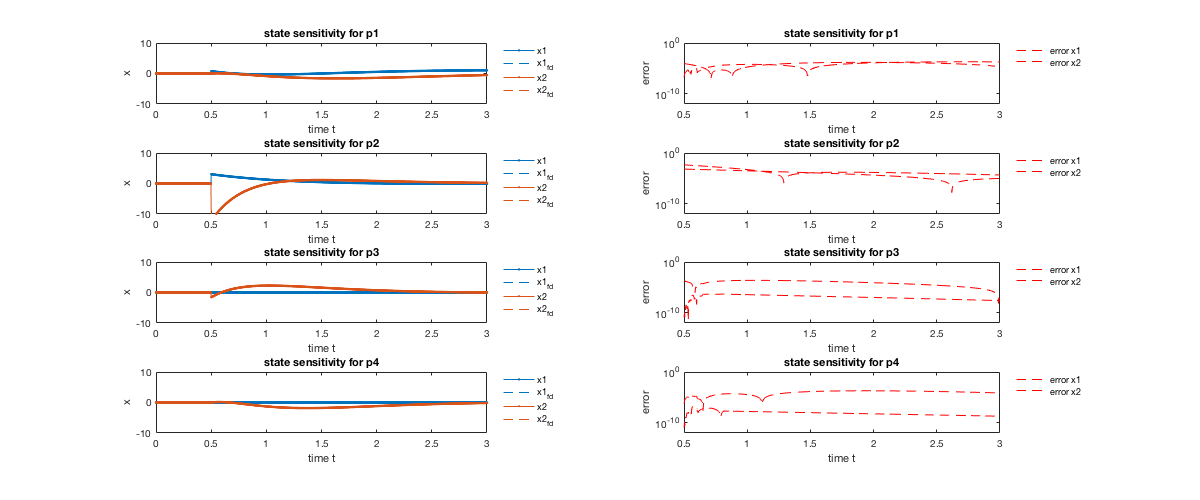
\includegraphics[width=\textwidth]{../../examples/example_dirac_secondorder_vectmult/html/example_dirac_secondorder_vectmult_01.png}

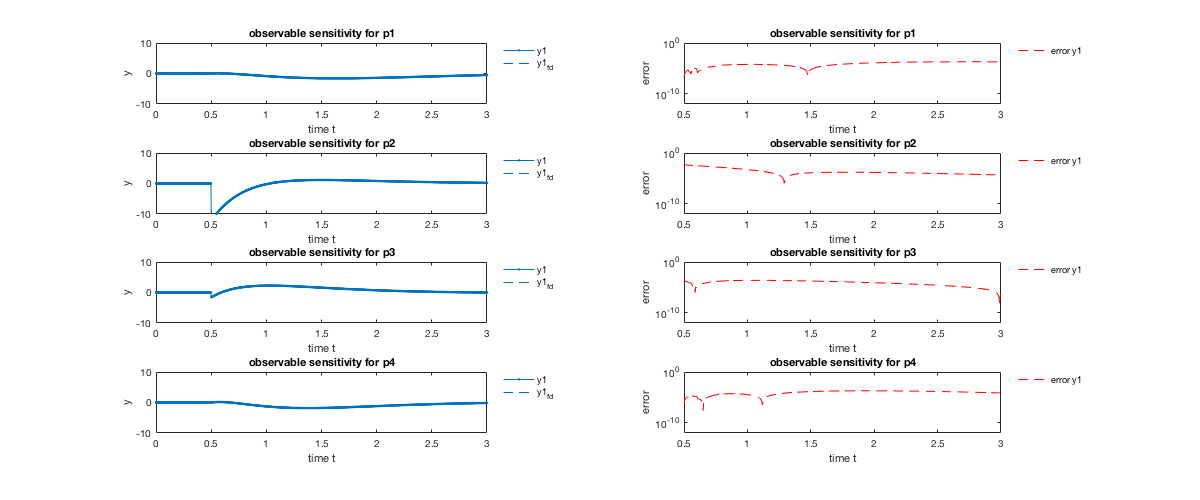
\includegraphics[width=\textwidth]{../../examples/example_dirac_secondorder_vectmult/html/example_dirac_secondorder_vectmult_02.png}
\begin{DoxyCode}
end
\end{DoxyCode}




    